\subsubsection{Leapfrog}

The Leapfrog solutions are in agreement with the expected results: both unfiltered and RAW-filtered solutions show an observed order of accuracy that tends to the formal $2^{nd}$ order. The two solutions are almost the same.

\begin{table}[!ht]
  \centering
  \caption{Oscillation test: errors analysis of explicit Leapfrog solvers}\label{tab:oscillation_errors_lf}
  \begin{subtable}[b]{0.40\textwidth}
    \centering
    \caption{Unfiltered}\label{tab:oscillation-leapfrog}
    \resizebox{1.00\textwidth}{!}{%
    \begin{tabular}{ccccc}
      \toprule
      {\sc Time Step} & {\sc Error X} & {\sc Error Y} & {\sc Order X} & {\sc Order Y} \\
      \hline
      5000.0          &  0.156E+02    &  0.156E+02    & /             & /             \\
      2500.0          &  0.849E+01    &  0.846E+01    & 0.87          & 0.88          \\
      1250.0          &  0.300E+01    &  0.303E+01    & 1.50          & 1.48          \\
       625.0          &  0.106E+01    &  0.107E+01    & 1.51          & 1.50          \\
       320.0          &  0.387E+00    &  0.392E+00    & 1.50          & 1.50          \\
       100.0          &  0.676E-01    &  0.685E-01    & 1.50          & 1.50          \\
      \bottomrule
    \end{tabular}}
  \end{subtable}\quad%
  \begin{subtable}[b]{0.40\textwidth}
    \centering
    \caption{RAW-filtered}\label{tab:oscillation-leapfrog-raw}
    \resizebox{1.00\textwidth}{!}{%
    \begin{tabular}{ccccc}
      \toprule
      {\sc Time Step} & {\sc Error X} & {\sc Error Y} & {\sc Order X} & {\sc Order Y} \\
      \hline
      5000.0          &  0.156E+02    &  0.156E+02    & /             & /             \\
      2500.0          &  0.855E+01    &  0.852E+01    & 0.86          & 0.87          \\
      1250.0          &  0.303E+01    &  0.305E+01    & 1.50          & 1.48          \\
       625.0          &  0.107E+01    &  0.108E+01    & 1.51          & 1.50          \\
       320.0          &  0.390E+00    &  0.395E+00    & 1.50          & 1.50          \\
       100.0          &  0.685E-01    &  0.692E-01    & 1.50          & 1.50          \\
      \bottomrule
    \end{tabular}}
  \end{subtable}\\
\end{table}

\begin{figure}[!ht]
  \centering
  \begin{subfigure}[b]{0.45\textwidth}
    \centering
    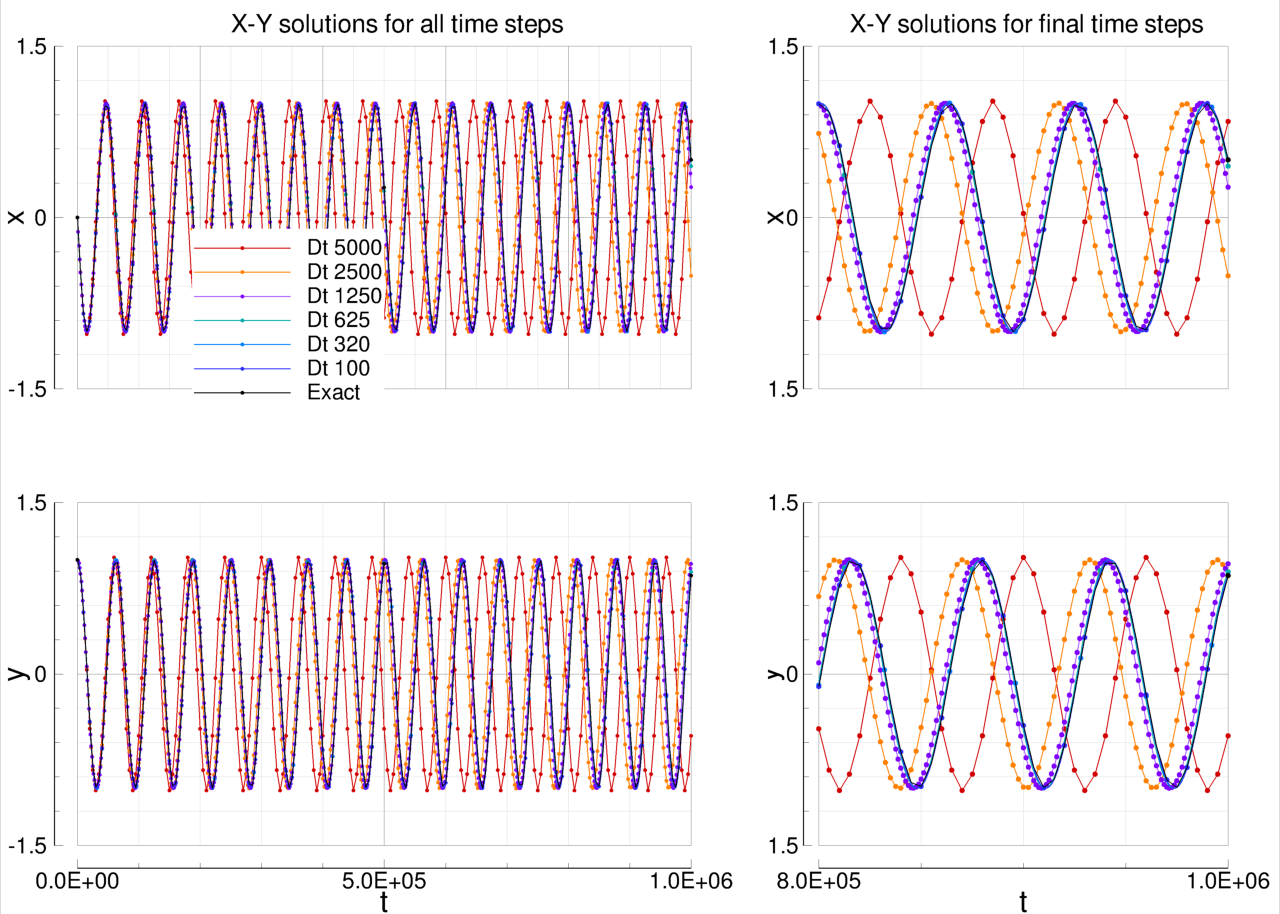
\includegraphics[width=1.00\textwidth]{errors-analysis/oscillation/errors_analysis-oscillation-leapfrog.png}
    \caption{Unfiltered}\label{fig:results-oscillation-leapfrog-unfiltered}
  \end{subfigure}\quad%
  \begin{subfigure}[b]{0.45\textwidth}
    \centering
    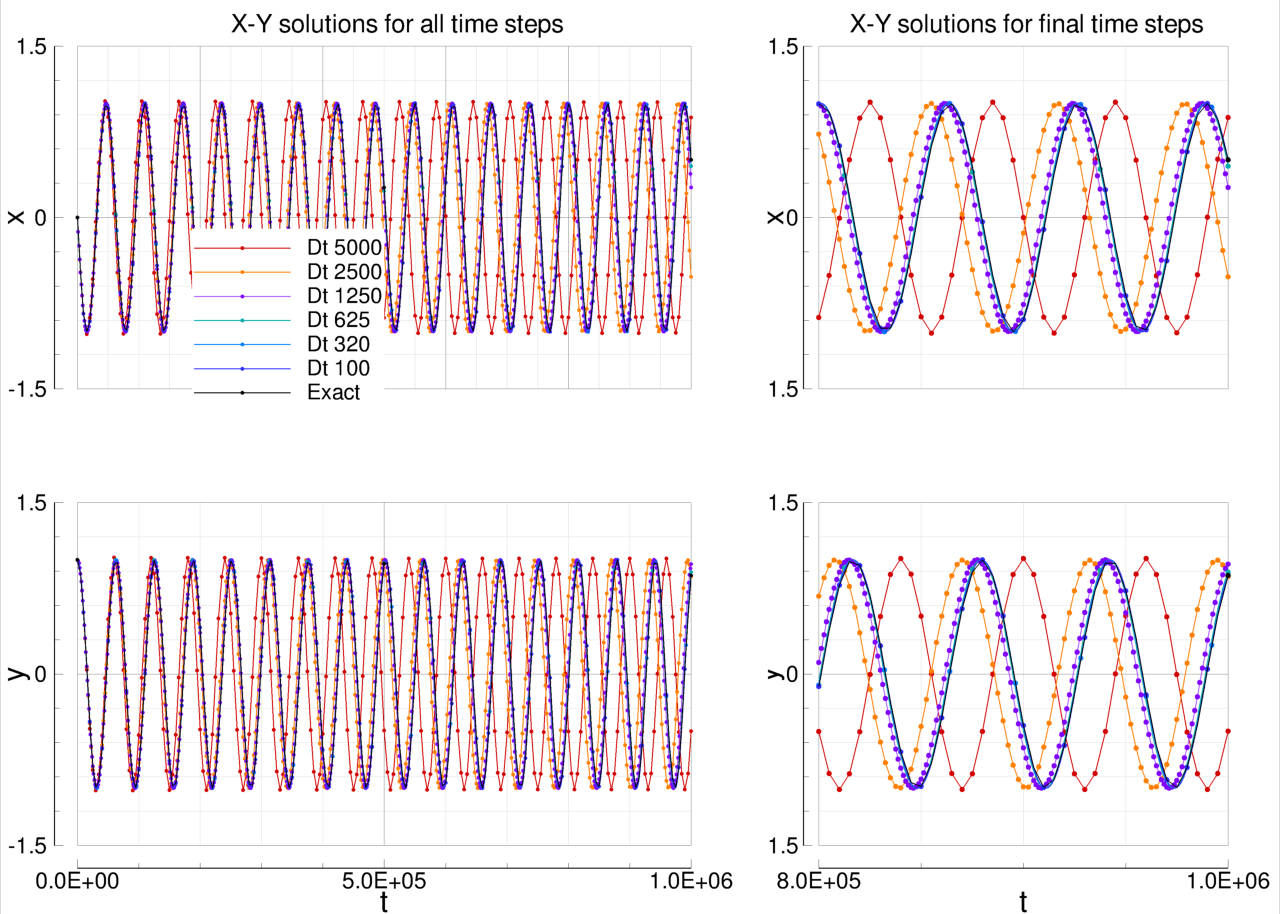
\includegraphics[width=1.00\textwidth]{errors-analysis/oscillation/errors_analysis-oscillation-leapfrog-raw.png}
    \caption{RAW-filtered}\label{fig:results-oscillation-leapfrog-raw}
  \end{subfigure}
  \caption{Oscillation equations solutions computed by means of Leapfrog solvers}\label{fig:results-oscillation-leapfrog}
\end{figure}

